% Discussion / AST
% Andreas
\section{AST}
\label{sect:discussion:ast}
In this section we will discuss the AST construction and output from our generated
parser. We will compare it to evaluated alternatives in section
\ref{sect:method:alternatives}, and we will discuss how it builds certain
constructs such as FLWOR and path expressions.

\subsection{Choice of structuring}
The rewrite rules and operators (described in section
\ref{sect:results:parser_output_ast}) made it easy to change and restructure the
AST output from ANTLR. In a intuitive way, they were used to construct subtrees
using both real and imaginary tokens, as described in section
\ref{sect:impl:ast}. Contrast this to JFlex/CUP, one of the alternative
parser generators evaluated in this project (see section
\ref{sect:method:alternatives}), where the AST construction has to be done
manually from scratch by adding action code to the grammar instead of simple
rewrite rules. However, this ease of change may makes it easy to break implicit
API contracts with other programs. A good starting point could be to study other
XQuery implementations and their respective AST structures. 

One notable problem with the rewrite rules in ANTLR is the fact that after they
have been added to the grammar, it is no longer possible to generate a parser
which does not produce an AST (by omitting the \verb!output=AST! option). ANTLR will
instead refuse to generate a parser and output syntax error messages since the rewrite
rules are no longer recognized.

The current AST output from ANTLR seems to be well suited for traversion and data
flow analysis, which is a requirement for implementation of type checking,
proper scoping and symbol tables, as well as optimizations and transformations
to new structures. ANTLR is capable of producing ``tree parsers'' (see
\cite{definitiveAntlr}, section 3.3) based on rewrite rules, so it may be
possible to utilize ANTLR even further to achieve a tree
parser without writing one from scratch.

In section \ref{sect:results:parser_output_ast}, we demonstrated the AST output
capabilities of our resulting parser. In figure \ref{tree:ast:flwor1}, an
example with a FLWOR query was presented. In this example there is a path
expression (\verb!/bookstore/book/title!, which is also used in the example in
figure \ref{tree:ast:pathexpr}) encoded as seen in figure
\ref{fig:discussion:ast:path1}. 

\begin{figure}[h!]
\centering
 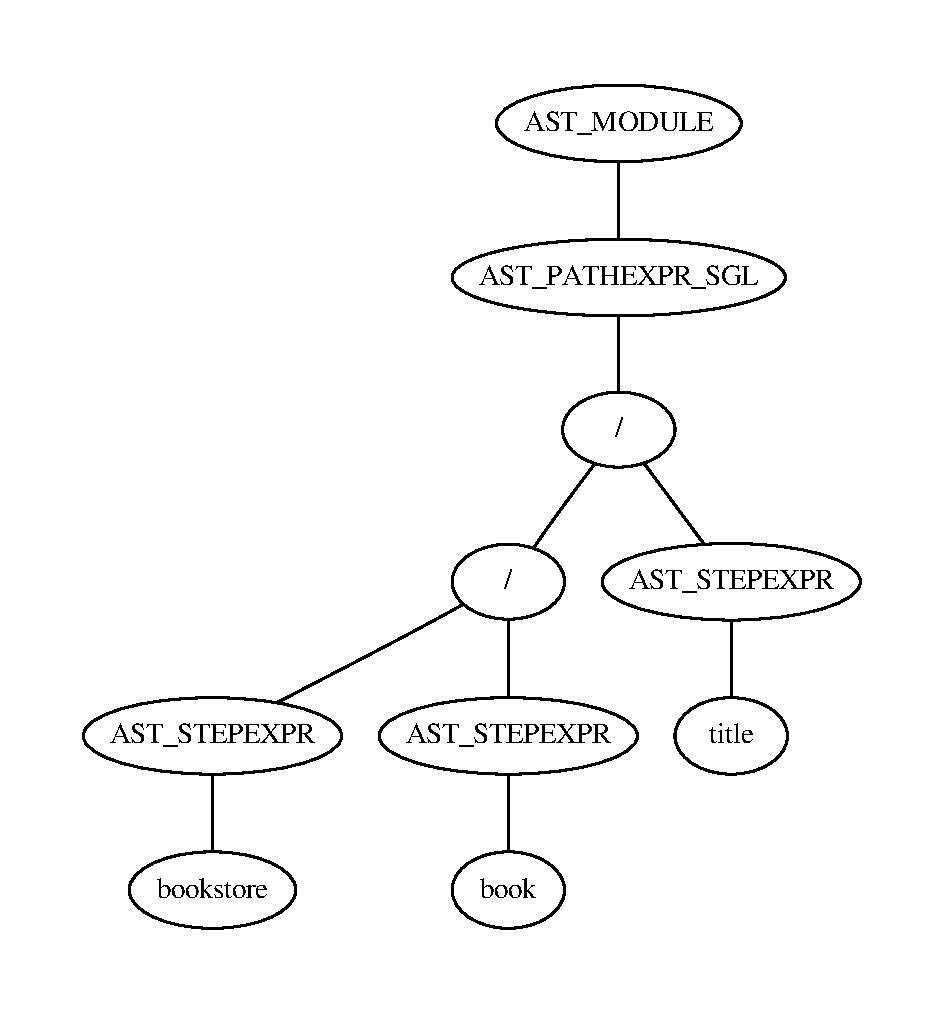
\includegraphics[width=0.4\textwidth]{img/graphs/path1}
\caption{Generated AST tree for a simple path expression}
\label{fig:discussion:ast:path1}
\end{figure}

This is one example of how to represent path expressions as tree structures.
With in-order tree traversal this tree should be fairly simple to reconstruct  
into the original path expression, as well as matching against a document object
model, or for performing staircase joins\cite{pathfinder_staircase}. Another  
proposed way to represent path expressions is the NoK (Next-of-Kin) tree
structure\cite{zhang_nok}, however NoK may be better suited for simple document
tree matching.

Further, the AST generated for a FLWOR query in figure \ref{tree:ast:flwor1}
(section \ref{sect:results:parser_output_ast}) can be represented in several
alternative ways that may be more fitted for loop-lifted staircase
joins\cite{pathfinder_staircase}. One such representation is
BlossomTree\cite{zhang_blossomtree}, which is tailored for representing
FLWOR-expressions which consists of multiple path expressions.

The representation of full-text queries is also a matter of interest. The
grammar is quite clear on operator and modifier precedence, however it may not
be obvious how to relate some modifiers (such as 
``\verb!with|without stemming!") to nodes. As seen in figure, we have simply
added this modifier as a sibling to the subject node. However, it could be
benefitial add this modifier as a child node of the subject node instead. This
is a recurring design question with regards to several other full-text
modifiers, and will need further research for optimum AST construction.

\subsection{Extendability and data flow analysis}
Currently the logic for scoping and symbol table lookups are embedded in the
grammar. It would be benefitial to have this logic removed and decoupled and
rather develop a data flow analysis framework with the necessary facilities for
performing scoping, symbol table lookup, as well as type inference and type
checking. The current implementation of scoping and symbol tables (described in
section \ref{sect:impl:scoping_and_symtab}) is adequate, however adding more
features could severly affect the readability and clarity of the grammar.

Generelle resultat, bra/d\aa rlig (AST) \#\# typesjekking (bedre \aa~gj\o re
p\aa~AST'en) -> putt i egen section i discussion -------v 
symtabs (bedre \aa~gj\o re p\aa~ AST'en))
 * Mulighet for dataflytanalyse, typesjekking, symboltabell

Gjorde vi riktige valg? Ble ting som forventet? Hva hadde skjedd om vi brukte alternativ m\aa te?

\underline{\textbf{\LARGE //ODOT:}}